\documentclass[a4paper,12pt]{article}
\usepackage[utf8]{inputenc}
\usepackage[brazil]{babel}
\usepackage{pdfpages}

\title{TCC---Relatório 1}
\author{Bernardo Bahia Monteiro \and Orientador: José Eduardo Mautone Barros}

\pagenumbering{gobble}

\begin{document}

\maketitle

\paragraph{Tema:} FADEC para uma mini turbina a gás aeronáutica

\paragraph{Resumo:} Desenvolvimento de um sistema de controle eletrônico do
motor (Full Authority Digital Engine Control---FADEC) para uma mini turbina a
gás aeronáutica. Inicialmente será desenvolvido um modelo dinâmico para a mini
turbina e os parâmetros do modelo serão estimados experimentalmente. Com esse
modelo, será desenvolvido um controlador que será testado por meio de simulações
computacionais e testes de laboratório usando o motor real.

O controlador deve ser capaz de realizar a partida do motor, controlar o aumento
e diminuição de potência usando um sinal de referência dado pelo piloto, e
desligar o motor. Durante o funcionamento, o controlador deve monitorar
possíveis falhas e garantir que o motor não exceda seu limite operacional

\paragraph{Cronograma:} O cronograma do trabalho está na página seguinte. Ele
não contempla a redação do trabalho, pois essa tarefa será feita de forma
concomitante ao desenvolvimento deste.

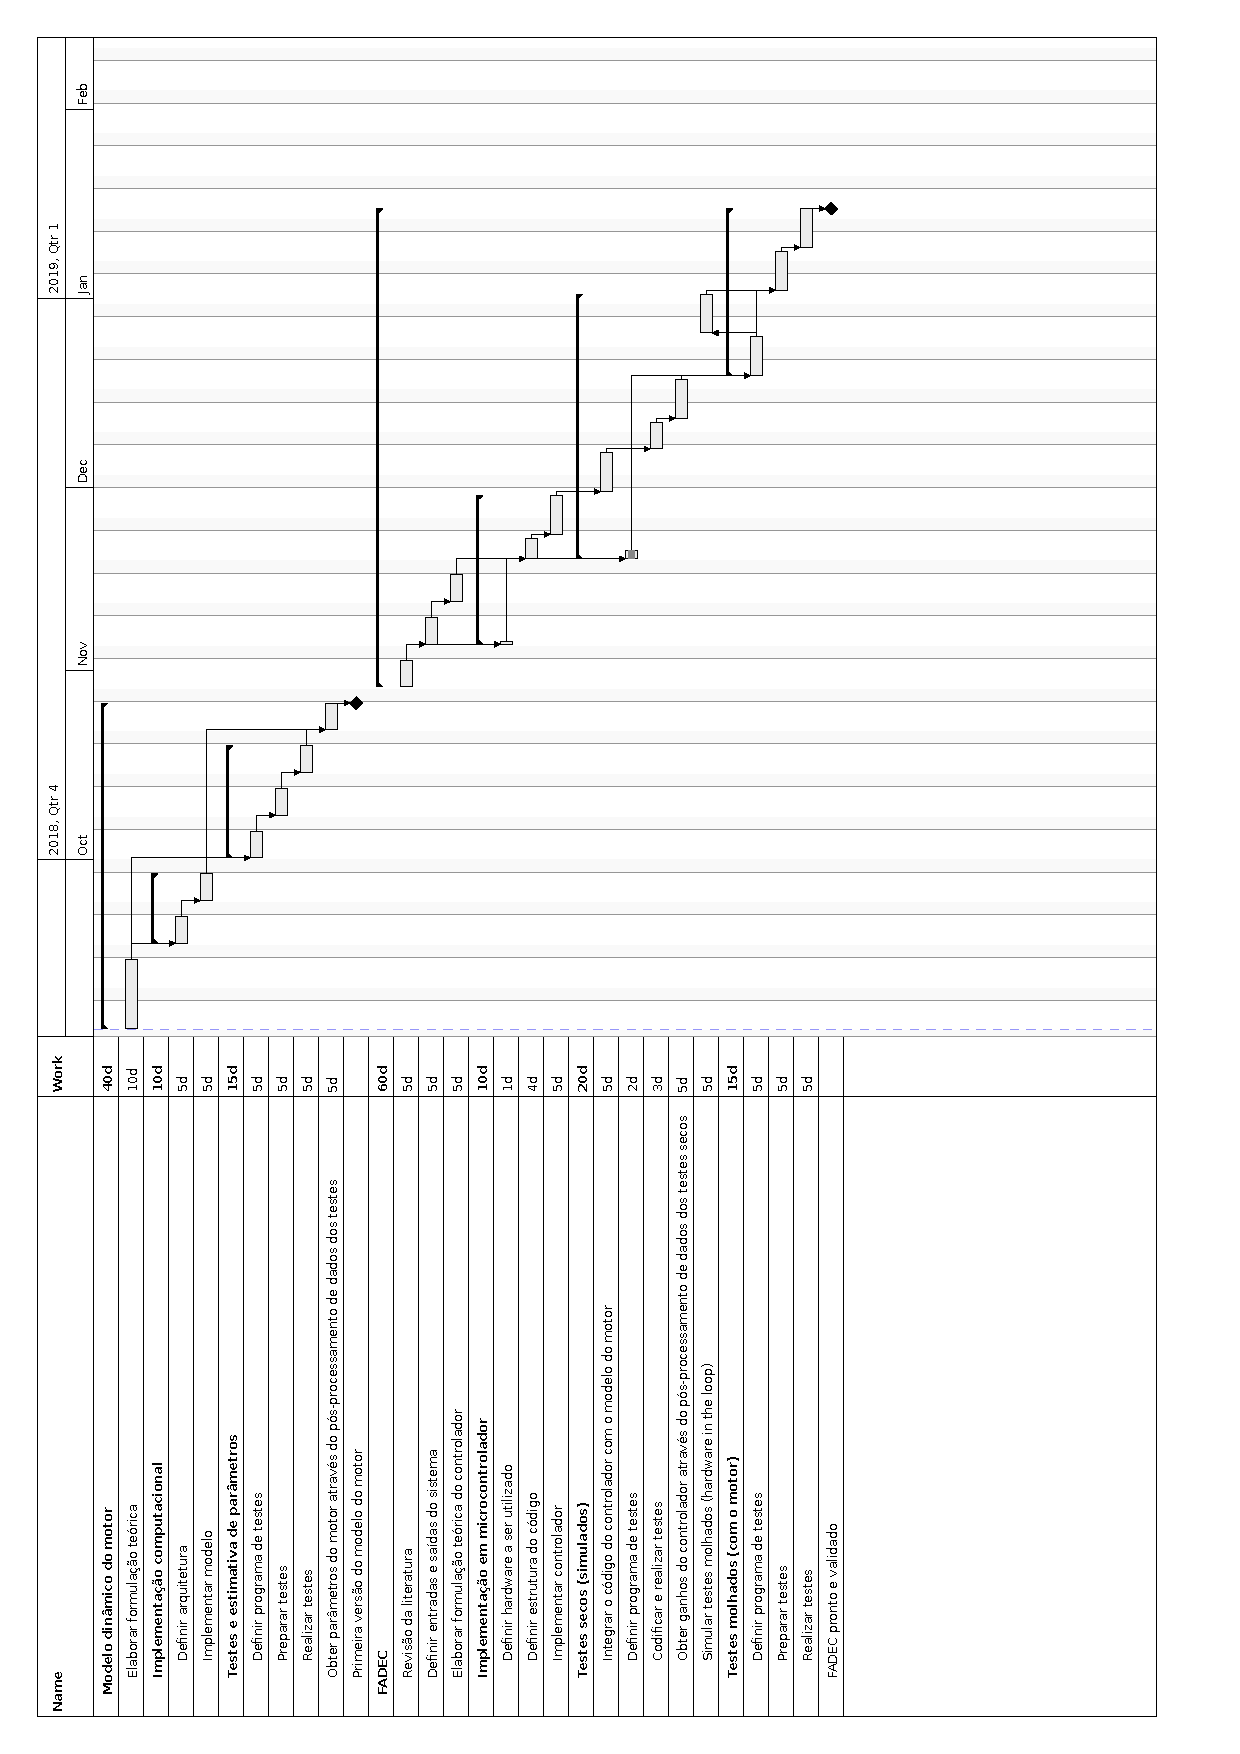
\includepdf[landscape,angle=-90]{gantt}

\end{document}
